\documentclass[tikz, preview]{standalone}
\usepackage{amsfonts, amsthm, amssymb, amsmath, stmaryrd, etoolbox}
\usepackage{tikz}
\usetikzlibrary{matrix,arrows}
\tikzset{->-/.style={decoration={markings, mark=at position .5 with {\arrow{>}}},postaction={decorate}}}
\tikzset{->-pos/.style={decoration={markings, mark=at position #1 with {\arrow{>}}},postaction={decorate}}}
\tikzset{->-/.style={decoration={markings,mark=at position .5 with {\arrow{>}}},postaction={decorate}}}
\tikzset{->-pos/.style={decoration={markings,mark=at position #1 with {\arrow{>}}},postaction={decorate}}}

\begin{document}
%%%%%%%%%%%%%%%%% 
%%%%%%%%%%%%%%%%% 
\[
  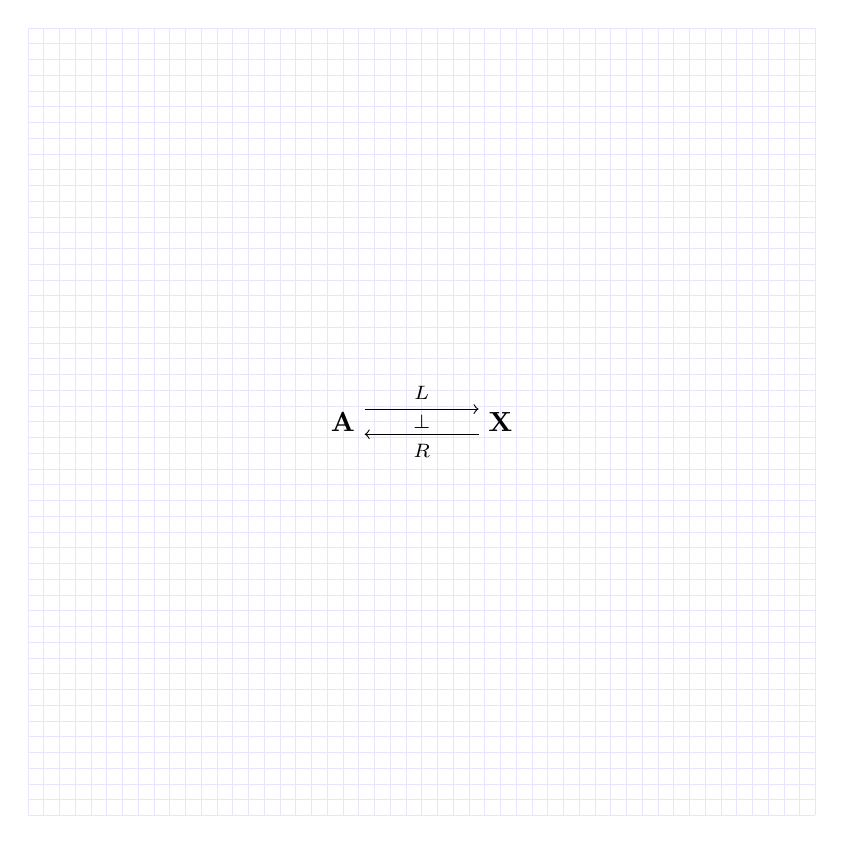
\begin{tikzpicture}
    \draw [help lines, step=0.2, color=blue!10] (-5,-5) grid (5,5); % grid
    % 
    \node (1) at (-1,0) {$ \mathbf{A} $};
    \node (2) at (1,0) {$ \mathbf{X} $};
    \node () at (0,0) {\scriptsize $ \perp $};
    \draw [->] (1.30) to node [above] {\scriptsize $ L $} (2.150);
    \draw [->] (2.-150) to node [below] {\scriptsize $ R $} (1.-30);
  \end{tikzpicture}
\]
%%%%%%%%%%%%%%%%% 
%%%%%%%%%%%%%%%%% 
\end{document}
